\documentclass[a4paper,12pt]{article}
\usepackage[utf8]{inputenc}
\usepackage[T2A]{fontenc}
\usepackage[russian]{babel}
\usepackage{amsmath,amssymb}
\usepackage{graphicx}
\usepackage{geometry}
\usepackage{listings}
\usepackage{xcolor}
% Для кликабельного содержания
\usepackage[hidelinks]{hyperref}
\geometry{left=2cm,right=2cm,top=2cm,bottom=2cm}

% Настройки для кода
\lstset{
  basicstyle=\ttfamily\small,
  keywordstyle=\color{blue},
  commentstyle=\color{gray},
  stringstyle=\color{purple},
  numbers=left,
  numberstyle=\tiny,
  breaklines=true,
  frame=single,
  rulecolor=\color{black!30},
  backgroundcolor=\color{black!5},
  showstringspaces=false
}

\begin{document}

% Титульный лист
\begin{titlepage}
  \begin{center}
    \textbf{Федеральное государственное}\\
    \textbf{автономное учебное учреждение высшего образования}\\[0.5em]
    \textbf{«Национальный исследовательский университет ИТМО»}\\[2em]
    \textbf{Мегафакультет компьютерных технологий и управления}\\
    \textbf{Факультет программной инженерии и компьютерной техники}\\[4em]
    \LARGE\textbf{Отчёт}\\[0.5em]
    \large по лабораторной работе №2\\
    по дисциплине «Вычислительная математика»\\[0.5em]
    \normalsize Вариант №4
  \end{center}

  \vfill
  \begin{flushright}
    Группа: P3207\\
    Студент: Исмоилов Шахзод Бахтиёрович\\
    Преподаватель: Рыбаков Степан Дмитриевич\\
  \end{flushright}

  \vspace{2em}
  \begin{center}
    Санкт-Петербург\\
    2025
  \end{center}
\end{titlepage}

% Оглавление
\tableofcontents
\newpage

% 1
\section{Цель лабораторной работы}
Изучить численные методы решения нелинейных уравнений и их систем, найти корни заданного нелинейного уравнения/системы нелинейных уравнений, выполнить программную реализацию методов.

% 2
\section{Задание}
Требования к программе:
\begin{itemize}Цель
  \item Все численные методы должны быть реализованы в виде отдельных подпроцессов/методов/классов.
  \item Пользователь выбирает уравнение, корень/корни которого требуется вычислить (3–5 функций, в том числе трансцендентные), из тех, которые предлагает программа.
  \item Предусмотреть ввод исходных данных (границы интервала/начальное приближение к корню и погрешность) из файла или с клавиатуры.
  \item Выполнить проверку исходных данных: проанализировать наличие корня на введённом интервале. При отсутствии корней выводить сообщение об ошибке.
  \item Для методов, требующих начального приближения (Ньютона, секущих, хорд с фиксированным концом, простой итерации) выбор начального приближения и проверку условия сходимости выполнять в программе.
  \item Предусмотреть вывод результатов (найденный корень, значение функции в корне, число итераций) в файл или на экран.
  \item Организовать вывод графика функции для всего исследуемого интервала (с запасом).
\end{itemize}

% 3
\section{Рабочие формулы использованных методов}
\subsection{Метод Ньютона (касательных)}
Пусть $y=f(x)$ на отрезке $[a,b]$. Инициализация: $x_0$ на отрезке $[a,b]$. В точке $x_{i-1}$ уравнение касательной:
\[ y = f(x_{i-1}) + f'(x_{i-1})(x - x_{i-1}). \]
Рабочая формула метода:
\[ x_i = x_{i-1} - \frac{f(x_{i-1})}{f'(x_{i-1})}. \]
Критерий остановки: $|x_n - x_{n-1}| \le \varepsilon$.

\subsection{Метод половинного деления}
Метод заключается в делении интервала пополам. На концах интервала $[a,b]$ функция имеет разные знаки. Рабочая формула:
\[ x_i = \frac{a_i + b_i}{2}. \]
Критерий остановки: $|x_n - x_{n-1}| \le \varepsilon$.

\subsection{Метод простой итерации}
Переписываем $f(x)=0$ в виде $x=\phi(x)$. Инициализация $x_0$ на отрезке $[a,b]$. Рабочая формула:
\[ x_{i+1} = \phi(x_i). \]
Условие сходимости: $|\phi'(x)| \le q < 1$ на $[a,b]$. Критерий остановки: $|x_n - x_{n-1}| \le \varepsilon$.

% 4
\section{Графики функций}
\subsection{Задание 1}
\begin{figure}[h!]
  \centering
  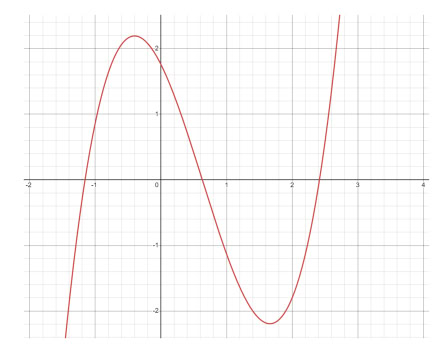
\includegraphics[width=0.8\textwidth]{fig1.png}
  \caption{График функции $x^3 - 1.89x^2 - 2x + 1.76$.}
\end{figure}

\subsection{Задание 2}
\begin{figure}[h!]
  \centering
  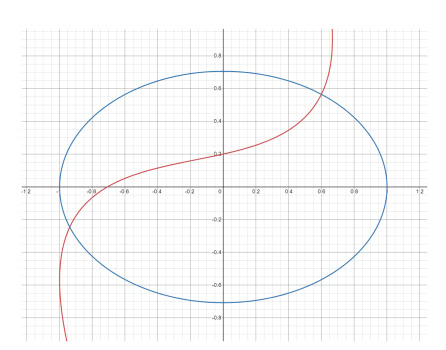
\includegraphics[width=0.8\textwidth]{fig2.png}
  \caption{График системы уравнений $\sin(x+y)-1.2x=0.2$ и $x^2+2y^2=1$.}
\end{figure}

% 5
\section{Заполненные таблицы вычислительной части №1}
Для функции $x^3 - 1.89x^2 - 2x + 1.76$:
\begin{enumerate}
  \item Графически отделены корни: $x_1=-1.156$, $x_2=0.63$, $x_3=2.416$.
  \item Интервалы изоляции:
    \begin{itemize}
      \item $[-2,0]$ для $x_1$
      \item $[0,2]$ для $x_2$
      \item $[2,4]$ для $x_3$
    \end{itemize}
  \item Точность $\varepsilon=0.01$.
\end{enumerate}

\subsection{Метод половинного деления для уточнения корня $x_1$}
\begin{table}[h!]
  \centering
  \begin{tabular}{|c|c|c|c|c|c|c|c|}
    \hline
    № & $a$ & $b$ & $x$ & $f(a)$ & $f(b)$ & $f(x)$ & $|a-b|$ \\
    \hline
    1 & -2    & 0     & -1.000 & -9.800 & 1.760 & 0.870  & 2 \\
    2 & -2    & -1    & -1.500 & -9.800 & 0.870 & -2.867 & 1 \\
    3 & -1.5  & -1    & -1.250 & -2.867 & 0.870 & -0.646 & 0.5 \\
    4 & -1.25 & -1    & -1.125 & -0.646 & 0.870 & 0.194  & 0.25 \\
    5 & -1.25 & -1.125& -1.188 & -0.646 & 0.194 & -0.208 & 0.125 \\
    6 & -1.188& -1.125& -1.157 & -0.208 & 0.194 & -0.005 & 0.063 \\
    7 & -1.157& -1.125& -1.141 & -0.005 & 0.194 & 0.096  & 0.032 \\
    8 & -1.157& -1.141& -1.149 & -0.005 & 0.096 & 0.046  & 0.016 \\
    9 & -1.157& -1.149& \textbf{-1.153} & -0.005 & 0.046 & 0.021  & 0.008 < \varepsilon \\
    \hline
  \end{tabular}
\end{table}

\subsection{Метод секущих для уточнения корня $x_2$}
\begin{table}[h!]
  \centering
  \begin{tabular}{|c|c|c|c|c|c|}
    \hline
    № & $x_{k-1}$ & $x_k$   & $x_{k+1}$  & $f(x_{k+1})$ & $|x_{k+1}-x_k|$ \\
    \hline
    1 & 0   & 1     & 0.609   & 0.06691 & 0.391 \\
    2 & 1   & 0.609 & 0.63086 & -0.00282 & 0.02186 \\
    3 & 0.609 & 0.63086 & \textbf{0.62997} & 0        & 0.00088 < \varepsilon \\
    \hline
  \end{tabular}
\end{table}

\subsection{Метод простой итерации для уточнения $x_3$}
\begin{table}[h!]
  \centering
  \begin{tabular}{|c|c|c|c|c|}
    \hline
    № & $x_k$   & $x_{k+1}$ & $f(x_{k+1})$ & $|x_{k+1}-x_k|$ \\
    \hline
    1 & 2.000 & 2.140 & -1.375 & 0.140 \\
    2 & 2.140 & 2.236 & -0.983 & 0.096 \\
    3 & 2.236 & 2.299 & -0.674 & 0.064 \\
    4 & 2.299 & 2.341 & -0.449 & 0.042 \\
    5 & 2.341 & 2.368 & -0.294 & 0.027 \\
    6 & 2.368 & 2.386 & -0.191 & 0.017 \\
    7 & 2.386 & 2.397 & -0.123 & 0.011 \\
    8 & 2.397 & \textbf{2.404} & -0.079 & 0.007 < \varepsilon \\
    \hline
  \end{tabular}
\end{table}

% 6 Решение системы
\section{Решение системы нелинейных уравнений \newline вычислительной части №2}
\subsection*{Левый корень}
Начальное приближение: $x_0=-0.94$, $y_0=-0.25$.\\
\textbf{Шаг 1.} Запишем систему для \(\Delta x,\Delta y\):
\[
\begin{cases}
\bigl(\cos(x+y)-\tfrac{6}{5}\bigr)\,\Delta x+\cos(x+y)\,\Delta y=\frac{x\cdot6}{5}+\frac15-\sin(x+y),\\
(2x)\,\Delta x+(4y)\,\Delta y= -2y^2+1-x^2.
\end{cases}
\]
На первой итерации система принимает вид:
\[
\begin{cases}
-0.82834\Delta x+0.37166\Delta y=0.00037,\\
-1.88\Delta x-1\Delta y=-0.0086.
\end{cases}
\]
\textbf{Шаг 2.} Решаем линейную систему: получаем $\Delta x=-0.06191$, $\Delta y=-0.26827$.\\
\textbf{Шаг 3.} Вычисляем новые приближения:
\[
x_1=x_0+\Delta x=-1.00191,\quad y_1=y_0+\Delta y=-0.26827.
\]
\textbf{Шаг 4.} Проверяем условие окончания при $\varepsilon=0.01$:
\[
|x_1-x_0|\le\varepsilon,\quad |y_1-y_0|>\varepsilon,
\]
продолжаем итерации (до \emph{Шага 12}), после чего получаем:
\[
x_3=-0.93813,\quad y_3=-0.24489.
\]

 \subsection*{Правый корень}
Начальное приближение: $x_0=0.6$, $y_0=0.5$.\
\textbf{Шаг 1.} Выбираем $x_0=0.6$, $y_0=0.5$. Исходная система:
\[
\begin{cases}
(\cos(x+y)-\tfrac{6}{5})\,\Delta x+(\cos(x+y))\,\Delta y=\frac{x\cdot6}{5}+\frac15-\sin(x+y),\
(2\cdot x)\,\Delta x+(4\cdot y)\,\Delta y=-2y^2+1-x^2.
\end{cases}
\]
\textbf{Шаг 2.} Решаем полученную систему. Получаем $\Delta x=0.00291$ и $\Delta y=0.06826$.\
\textbf{Шаг 3.} Вычисляем очередные приближения:
\[
 x_1=x_0+\Delta x=0.6+0.00291=0.60291,\
 y_1=y_0+\Delta y=0.5+0.06826=0.56826.
\]
\textbf{Шаг 4.} Проверяем критерии окончания при $\varepsilon=0.01$:
\[
|x_1-x_0|\le\varepsilon\quad и \quad|y_1-y_0|\le\varepsilon,\
|0.60291-0.6|\le\varepsilon\quad и \quad|0.56826-0.5|>\varepsilon.
\]
\textbf{Шаг 5.} Подставляем очередные приближения в систему:
\[
\begin{cases}
-0.81092\Delta x+0.38908\Delta y=0.00228,\
1.20581\Delta x+2.27303\Delta y=-0.00933.
\end{cases}
\]
\textbf{Шаг 6.} Решаем полученную систему. Получаем $\Delta x=-0.00381$ и $\Delta y=-0.00208$.\
\textbf{Шаг 7.} Вычисляем очередные приближения:
\[
 x_2=x_1+\Delta x=0.60291-0.00381=0.59909,\
 y_2=y_1+\Delta y=0.56826-0.00208=0.56618.
\]
\textbf{Шаг 8.} Проверяем критерии окончания при $\varepsilon=0.01$:
\[
|x_2-x_1|\le\varepsilon\quad и \quad|y_2-y_1|\le\varepsilon,\
|0.59909-0.60291|\le\varepsilon\quad и \quad|0.56618-0.56826|\le\varepsilon.
\]
% 7 Листинг программы
\section{Листинг программы}

\subsection*{Метод половинного деления}
\begin{lstlisting}[language=Python, caption=Листинг: Метод половинного деления]
def half_method(quation, method):
    a, b, inaccuracy = input_selection(quation, method)

    iterations = 1
    max_iter = 10000

    if (float(b) - float(a) - 0.00001 < 0):
        print("Правая граница должна быть больше левой границы!")
        exit()

    count_roots = count_roots_on_interval(quation, a, b, 0.001)
    if not validate_roots(count_roots):
        exit()

    a1, b1 = a, b
    iterations = 1
    max_iter = 1000
    while (b - a) / 2 > inaccuracy and iterations < max_iter:
        midpoint = (a + b) / 2
        if quation_solution(quation, midpoint) == 0:
            return midpoint, iterations
        elif quation_solution(quation, a) * quation_solution(quation, midpoint) < 0:
            b = midpoint
        else:
            a = midpoint
        iterations += 1
    if iterations >= max_iter - 1:
        print("Решение не найдено")
        exit()

    solution = try_to_convert_to_int((a + b) / 2)
    print(f"Ответ = {solution}")
    print(f"f(ответ) = {quation_solution(quation, solution)}")
    print(f"Итерации = {iterations}")
    output_data(solution, quation_solution(quation, solution), iterations, str_quation(quation))
    draw_grapth(quation, str_quation(quation), a1, b1, solution, quation_solution(quation, solution))
\end{lstlisting}

\subsection*{Метод Ньютона}
\begin{lstlisting}[language=Python, caption=Листинг: Метод Ньютона]
def Newton_method(quation, method):
    a, b, inaccuracy = input_selection(quation, method)

    approximation = validate_initial_approximation(quation, a, b)

    iterations = 1
    max_iter = 1000
    x = approximation
    while abs(quation_solution(quation, x)) > inaccuracy and iterations < max_iter:
        x = x - quation_solution(quation, x) / quation_df_solution(quation, x)
        iterations += 1

    solution = try_to_convert_to_int(x)
    output_data(solution, quation_solution(quation, solution), iterations, str_quation(quation))
    draw_grapth(quation, str_quation(quation), a, b, solution, quation_solution(quation, solution))
\end{lstlisting}

\subsection*{Метод простой итерации (уравнения)}
\begin{lstlisting}[language=Python, caption=Листинг: Метод простой итерации]
def Simple_iteration_method(quation, method):
    a, b, inaccuary = input_selection(quation, method)
    q = check_convergencecondition(quation, a, b)
    approximation = validate_initial_approximation(quation, a, b)
    x = approximation
    iterations = 1
    max_iter = 1000
    if q > 1:
        print("Условие сходимости НЕ выполнено")
        exit()
    elif 0 < q <= 0.5:
        while abs(converted_quation(quation, x) - x) > inaccuary and iterations < max_iter:
            x = converted_quation(quation, x)
            iterations += 1
    else:
        while abs(converted_quation(quation, x) - x) > ((1 - q) / q) * inaccuary and iterations < max_iter:
            x = converted_quation(quation, x)
            iterations += 1

    solution = try_to_convert_to_int(x)
    output_data(solution, quation_solution(quation, solution), iterations, str_quation(quation))
    draw_grapth(quation, str_quation(quation), a, b, solution, quation_solution(quation, solution))
\end{lstlisting}

\subsection*{Метод простой итерации (системы)}
\begin{lstlisting}[language=Python, caption=Листинг: Метод простой итерации для систем]
def simple_iteration_method(system, method):
    x0 = choose_x()
    y0 = choose_y()
    inaccuracy = choose_inaccuracy()
    max_iter = 1000
    iteration = 1

    if not check_convergence(system, method, x0, y0):
        print("Итерационная матрица не удовлетворяет условию сходимости.")
        return

    for _ in range(max_iter):
        x = f1(x0, y0, system)
        y = f2(x0, y0, system)
        if abs(x - x0) < inaccuracy and abs(y - y0) < inaccuracy:
            print(f"x = {x}, y = {y}, iterations = {iteration}")
            break
        x0, y0 = x, y
        iteration += 1
    output_data(x0, y0, f1(x, y, system), iteration)
\end{lstlisting}
Ссылка на проект: \url{https://github.com/Djerden/computation-math/tree/main/lab2}

% 8
% 8 Результаты
\section{Результаты выполнения программы}
\begin{verbatim}
Выберите вариант:
1) Нелинейное уравнение
2) Система нелинейных уравнений
1
Выберите уравнение:
1) x^2 - 3x + 2 
2) x^3 + 2x^2 - 5
3) cos(x) - x^2
1
Выберите метод:
1) Метод половинного деления
2) Метод Ньютона
3) Метод простой итерации
1
Выберите ввод:
1) Ввод вручную 
2) Ввод из файла
1
Введите левую границу интервала: 1
Введите правую границу интервала: 5
Введите точность: 0.01     
Ответ = 4.9921875
f(ответ) = 11.94537353515625
Итерации = 9
Выберите формат вывода:
1) В консоль
2) В файл
1
Уравнение: x^2 - 3x + 2  
Решение: 4.9921875 
f(4.9921875) =  11.94537353515625 
Итерации: 9
\end{verbatim}

Также в интерфейсе matplotlib отображается график решения (пример):

\begin{figure}[h!]
  \centering
  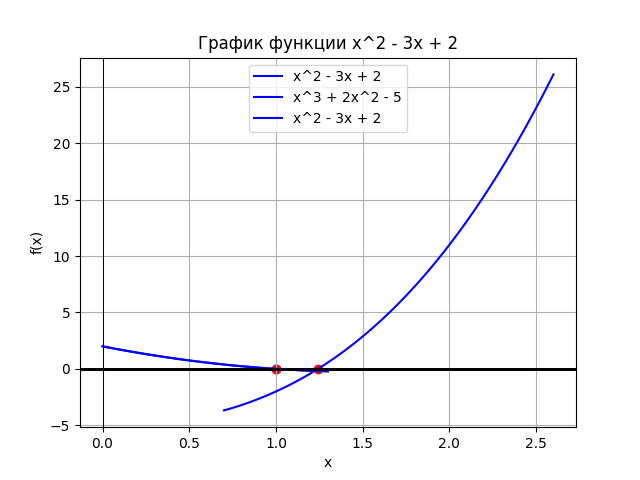
\includegraphics[width=0.7\textwidth]{fig3.png}
  \caption{График функции $x^2 - 3x + 2$ с найденным корнем.}
\end{figure}

% 9
\section{Вывод}
В работе были рассмотрены и реализованы три метода поиска корней нелинейных уравнений:
\begin{itemize}
  \item Метод половинного деления (дихотомии).
  \item Метод Ньютона (касательных).
  \item Метод простой итерации.
\end{itemize}

Для каждого метода были проведены следующие этапы:
\begin{enumerate}
  \item Выбор и проверка исходных данных (интервала или начального приближения).
  \item Итерационный процесс до достижения заданной точности $\varepsilon$.
  \item Вывод найденного корня, значения функции в корне и числа итераций.
  \item Построение графика функции с выделенным корнем.
\end{enumerate}

Сравнительный анализ методов:
\begin{itemize}
  \item Метод дихотомии гарантированно сходится при наличии корня на интервале, однако скорость сходимости линейная: $n \approx \log_2\frac{b-a}{\varepsilon}$.
  \item Метод Ньютона обладает квадратичной скоростью сходимости при выполнении условия дифференцируемости функции и правильного выбора начального приближения.
  \item Метод простой итерации имеет скорость сходимости, зависящую от коэффициента Липшица $q < 1$.
\end{itemize}

Работа демонстрирует практическую реализацию численных методов и их сравнение по критериям сходимости и точности.

\end{document}\end{document}
